\documentclass[a4paper, 12pt]{article}		% general format
\usepackage{multicol}
%%%% Charset
\usepackage{cmap}							% make PDF files searchable and copyable
\usepackage[utf8x]{inputenc} 				% accept different input encodings
\usepackage[english,russian]{babel}   %% загружает пакет многоязыковой вёрстки
\usepackage{fontspec}      %% подготавливает загрузку шрифтов Open Type, True Type и др.
\defaultfontfeatures{Ligatures={TeX},Renderer=Basic}  %% свойства шрифтов по умолчанию
\setmainfont[Ligatures={TeX,Historic}]{Roboto-Light} %% задаёт основной шрифт документа
\setsansfont{Roboto-Light}  
\usepackage{float}
%%%% Graphics
\usepackage[dvipsnames]{xcolor}			% driver-independent color extensions
\usepackage{graphicx}						% enhanced support for graphics
\usepackage{wrapfig}						% produces figures which text can flow around
\usepackage{hyperref}
%%%% Math
\usepackage{amsmath}						% American Mathematical Society (AMS) math facilities
\usepackage{amsfonts}						% fonts from the AMS
\usepackage{amssymb}						% additional math symbols

%%%% Typograpy (don't forget about cm-super)
\usepackage{microtype}						% subliminal refinements towards typographical perfection
\linespread{1.3}							% line spacing
\usepackage[left=2.5cm, right=1.5cm, top=2.5cm, bottom=2.5cm]{geometry}
\setlength{\parindent}{0pt}					% we don't want any paragraph indentation
\usepackage{parskip}						% some distance between paragraphs

%%%% Tables
\usepackage{tabularx}						% tables with variable width columns
\usepackage{multirow}						% for tabularx
\usepackage{hhline}							% for tabularx
\usepackage{tabu}
\usepackage{longtable}

%%%% Graph
\usepackage{tikz}							% package for creating graphics programmatically
\usetikzlibrary{arrows}						% edges for tikz

%%%% Other
\usepackage{url}							% verbatim with URL-sensitive line breaks
\usepackage{fancyvrb}						% sophisticated verbatim text (with box)

\usepackage{listings}
\usepackage{caption}
\DeclareCaptionFont{white}{\color{white}}
\DeclareCaptionFormat{listing}{\colorbox{gray}{\parbox{\dimexpr\textwidth-1.72\fboxsep\relax}{#1#2#3}}}
\captionsetup[lstlisting]{format=listing,labelfont=white,textfont=white,margin=0pt}
\lstset{language=C,
	basicstyle=\footnotesize,
	keepspaces=true,
	tabsize=4,               
	frame=single,                           % Single frame around code
	rulecolor=\color{black},
	captionpos=b,
	showstringspaces=false,	
	abovecaptionskip=-0.9pt,
	xleftmargin=3.4pt,
	xrightmargin=2.6pt,
	breaklines=true,
	postbreak=\raisebox{0ex}[0ex][0ex]{\ensuremath{\color{black}\hookrightarrow\space}},
	xleftmargin=3.2pt,
	literate={а}{{\selectfont\char224}}1
	{~}{{\textasciitilde}}1
	{б}{{\selectfont\char225}}1
	{в}{{\selectfont\char226}}1
	{г}{{\selectfont\char227}}1
	{д}{{\selectfont\char228}}1
	{е}{{\selectfont\char229}}1
	{ё}{{\"e}}1
	{ж}{{\selectfont\char230}}1
	{з}{{\selectfont\char231}}1
	{и}{{\selectfont\char232}}1
	{й}{{\selectfont\char233}}1
	{к}{{\selectfont\char234}}1
	{л}{{\selectfont\char235}}1
	{м}{{\selectfont\char236}}1
	{н}{{\selectfont\char237}}1
	{о}{{\selectfont\char238}}1
	{п}{{\selectfont\char239}}1
	{р}{{\selectfont\char240}}1
	{с}{{\selectfont\char241}}1
	{т}{{\selectfont\char242}}1
	{у}{{\selectfont\char243}}1
	{ф}{{\selectfont\char244}}1
	{х}{{\selectfont\char245}}1
	{ц}{{\selectfont\char246}}1
	{ч}{{\selectfont\char247}}1
	{ш}{{\selectfont\char248}}1
	{щ}{{\selectfont\char249}}1
	{ъ}{{\selectfont\char250}}1
	{ы}{{\selectfont\char251}}1
	{ь}{{\selectfont\char252}}1
	{э}{{\selectfont\char253}}1
	{ю}{{\selectfont\char254}}1
	{я}{{\selectfont\char255}}1
	{А}{{\selectfont\char192}}1
	{Б}{{\selectfont\char193}}1
	{В}{{\selectfont\char194}}1
	{Г}{{\selectfont\char195}}1
	{Д}{{\selectfont\char196}}1
	{Е}{{\selectfont\char197}}1
	{Ё}{{\"E}}1
	{Ж}{{\selectfont\char198}}1
	{З}{{\selectfont\char199}}1
	{И}{{\selectfont\char200}}1
	{Й}{{\selectfont\char201}}1
	{К}{{\selectfont\char202}}1
	{Л}{{\selectfont\char203}}1
	{М}{{\selectfont\char204}}1
	{Н}{{\selectfont\char205}}1
	{О}{{\selectfont\char206}}1
	{П}{{\selectfont\char207}}1
	{Р}{{\selectfont\char208}}1
	{С}{{\selectfont\char209}}1
	{Т}{{\selectfont\char210}}1
	{У}{{\selectfont\char211}}1
	{Ф}{{\selectfont\char212}}1
	{Х}{{\selectfont\char213}}1
	{Ц}{{\selectfont\char214}}1
	{Ч}{{\selectfont\char215}}1
	{Ш}{{\selectfont\char216}}1
	{Щ}{{\selectfont\char217}}1
	{Ъ}{{\selectfont\char218}}1
	{Ы}{{\selectfont\char219}}1
	{Ь}{{\selectfont\char220}}1
	{Э}{{\selectfont\char221}}1
	{Ю}{{\selectfont\char222}}1
	{Я}{{\selectfont\char223}}1,
	extendedchars=true
}

%галочка
\usepackage{amssymb}% http://ctan.org/pkg/amssymb
\usepackage{pifont}% http://ctan.org/pkg/pifont
\newcommand{\cmark}{\ding{52}}%
\newcommand{\xmark}{\ding{56}}
%------------------------------------------------------------------------------
\renewcommand{\labelenumii}{\theenumii}
\renewcommand{\theenumii}{\theenumi.\arabic{enumii}.}
\begin{document}
%------------------------------------------------
	\begin{titlepage}
		\begin{center}
			\large {Санкт-Петербургский политехнический университет Петра Великого\\
				Институт компьютерных наук и технологий}\\
		\end{center}
		\begin{center}
			\large\textbf {Кафедра компьютерных систем и программных технологий}
		\end{center}
		\vfill
		\begin{center}
			\large{\textbf{Отчет о лабораторной работе №5} \\
			\textbf{Курс: } Администрирование компьютерных сетей\\
			\textbf{Тема: } Перенос сети в Cisco Packet Tracer}
		\end{center}
		
		\vfill
		
		\flushleft{Выполнил студент группы 13541/3} 
		\hfill\parbox{9 cm}{\hspace*{3cm}\hbox to 0cm{\raisebox{-1em}{\small(подпись)}}\hspace*{-0.8cm}\rule{3cm}{0.8pt} Д.В. Круминьш}\\[0.6cm]
		
		\flushleft{Преподаватель} \hfill\parbox{9 cm}{\hspace*{3cm}\hbox to 0cm{\raisebox{-1em}{\small(подпись)}}\hspace*{-0.8cm}\rule{3cm}{0.8pt} И.А. Малышев}\\[0.6cm]
		
		\vspace{\fill}
		\begin{center}
			Санкт-Петербург \\ 2018 г.
		\end{center}
	\end{titlepage}
%------------------------------------------------
\setcounter{page}{2}
\tableofcontents
\clearpage

%------------------------------------------------------------------------------
%\input{intro}
\section{Введение}
\subsection{Назначение}
Целью данного документа является дать детальное описание к разрабатываемой операционной системе - \textbf{ReactOS}. Документ иллюстрирует цель и полную спецификацию для разработки продутка. В нем также приведены системные ограничения, интерфейсы и взаимодействие с другими внешними приложениями.


\subsection{Область применения}
\textbf{Идентификация продукта} - ReactOS.\\\\
Концептуальные принципы:
\begin{itemize}
\item \textbf{Совместимость.} ОС имеет привычный интерфейс пользователя семейства Windows, поддерживает файловые системы FAT16,FAT32,NTFS. Подавляющее большинство приложений, разработанных под MS DOS,Windows 9x/NT4/2000, а также некоторые программы под OS/2 и POSIX.
\item \textbf{Переносимость.} ОС работает на различных 32-разрядных процессорах семействах x86 производства компаний Intel и AMD. Возможна реализация поддержки процессоров других архитектур.
\item \textbf{Масштабируемость.} В ОС реализована поддержка технологий работы в многопроцессорных системах (SMP и COW(Cluster оf Workstations)).
\item \textbf{Распределённая обработка.} ОС имеет встроенные в систему сетевые возможности, обеспечивающие реализацию связи с различными типами компьютеров-хостов благодаря наличию разнообразных транспортных протоколов и технологии «клиент-сервер».
\item \textbf{Универсальность.} ОС содержит множество стандартных встроенных приложений пользовательского и служебного назначения, позволяющих начать эксплуатацию компьютера даже без постановки внешних приложений.
\item \textbf{Быть свободной и бесплатной} операционной системы с открытым кодом;
\item \textbf{Не нарушать патентов} на интеллектуальную собственность.
\end{itemize}

Целевая аудитория:
\begin{itemize}
\item Пользовательский сектор;
\begin{itemize}
\item Использование продукта в качестве домашней ОС, и в профессиональной деятельности в качестве рабочей ОС.
\end{itemize}
\item Серверный сектор.
\begin{itemize}
\item Оптимизация для Web-служб и Web-узлов;
\item Ориентация на малый, средний и крупный бизнес (большой объем оперативной памяти(до 32 гигабайт), безперебойная работа при большой нагрузке).
\end{itemize}
\end{itemize}

Выгода от использования \textbf{ReactOS} в отличии от \textbf{Windows Server 2003} заключается в том, что нет необходимости оплаты лицензии за использование ОС, при сохранении полной функциональности ОС.

В будущем предполагается полное вытеснение ОС семейства Windows.

\subsection{Определения, акронимы и сокращения}
\tabulinesep = 1mm
\begin{longtabu} to \textwidth {|X[2, m ] |X[6, l, m ] |}\firsthline\hline
\textbf{Термин}&\textbf{Определение}\\ \hline \endfirsthead
Пользователь	&Кто-то, кто взаимодействует с продуктом\\ \hline
Режим ядра & Уровень, на котором осуществляется доступ к системным данным и аппаратному обеспечению. \\ \hline
Исполнительная система& Объединяет в себе все службы управления. \\ \hline
Plug and Play& Технология, предназначенная для быстрого определения и конфигурирования устройств. \\ \hline
Аппаратно-зависимый уровень (HAL)& Это абстрактный уровень, расположенный над реальным оборудованием, через который проходят все обращения к аппаратным устройствам. \\ \hline
\caption{Определения терминов}
\end{longtabu}

\tabulinesep = 1mm
\begin{longtabu} to \textwidth {|X[6, m ] |X[2, l, m ] |}\firsthline\hline
\textbf{Термин}&\textbf{Акроним}\\ \hline \endfirsthead
Диспетчер виртуальной памяти (Virtual Memory Manager& VMM \\ \hline
Аппаратно-зависимый уровень (Hardware Abstraction Layer)& HAL \\ \hline
Интерфейс графического устройства (Graphical Device Interface) & GDI \\ \hline
Архитектура симметричной многопроцессорности (Symmetric Multiprocessing)& SMP \\ \hline
\caption{Таблица акронимов}
\end{longtabu}

\subsection{Ссылки}
$[$1$]$ Джоел Скамбрэй, Стюарт Макклури. Секреты хакеров. Безопасность Microsoft Windows Server 2003\\
$[$2$]$ С.В. Симонович, Г.А. Евсеев. Эффективный справочник 416 С. 2006\\
$[$3$]$ Ренд Моримото, Кентон Гардиньер. Microsoft Windows Server 2003 Полное руководство.\\
$[$4$]$ Станек У.Р. - Windows Server 2003. Справочник администратора\\
$[$5$]$ М.Руссинович, Д.Соломон. Внутреннее устройство Microsoft Windows\\
$[$6$]$ Джон Поль Мюллер, Питер Нортон. Полное руководство по Microsoft Windows XP


\section{Общее описание}
\subsection{Позиционирование продукта}
Архитектура ReactOS включает в себя два основных уровня — пользовательский режим (user mode) и режим ядра (kernel mode).
\begin{figure}[H]
  \centering
  \fbox{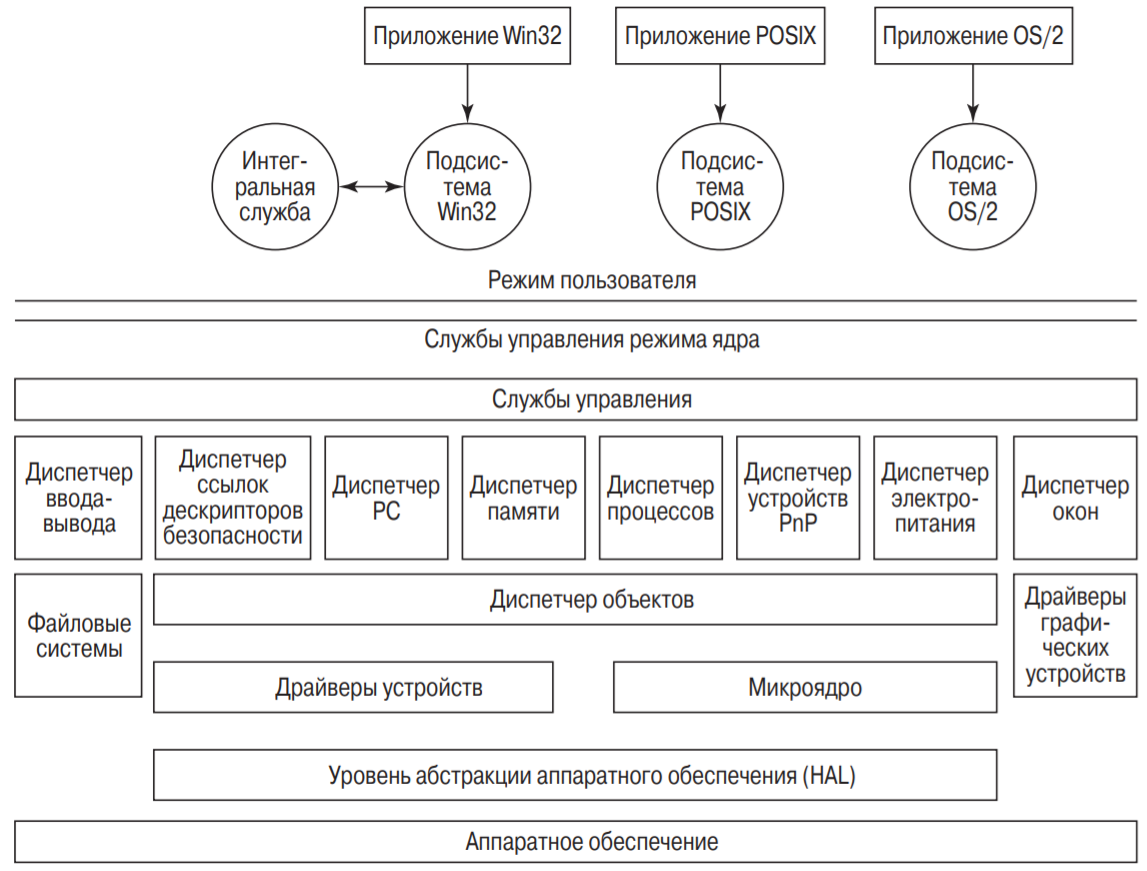
\includegraphics[width=\textwidth]{img/app_int}}
  \caption{Архитектура операционной системы ReactOS}
\end{figure}
\subsubsection{Режим пользователя}
Пользовательский режим представляет собой уровень поддержки приложений, состоящий из подсистем среды и интегральных подсистем. Именно в этой части операционной системы сторонние производители программного обеспечения могут выполнять системные вызовы готовых интерфейсов API и объектно-ориентированных компонентов. Все приложения и службы устанавливаются на уровне пользовательского режима.
\subsubsubsection{Подсистемы среды}
Подсистемы среды (environment subsystems) обеспечивают возможность запуска приложений, написанных для различных операционных систем. Подсистемы среды перехватывают вызовы приложений, обращенные к интерфейсу API конкретной операционной системы, и преобразуют эти вызовы в формат, понятный ReactOS. Затем преобразованные вызовы интерфейсов API передаются компонентам операционной системы, обрабатывающим запросы. 
\tabulinesep = 1mm
\begin{longtabu} to \textwidth {|X[l, m ] |X[2, l, m ] |}\firsthline\hline
\textbf{Подсистемная среда}&\textbf{Назначение}\\ \hline \endfirsthead
Windows Server 2003 Win32 (32-разрядная)&Поддерживает приложения Win32, а также отвечает за поддержку 16-разрядных приложий Windows и DOS. Данная подсистема обрабатывает все операции ввода-вывода в приложениях и функциях графического интерфейса поёьзователя\\ \hline
OS/2 & Поддерживает 16-разрядные приложения OS/2 (преимуществен Microsoft OS/2)\\ \hline
POSIX&Поддерживает POSIX-совместимые приложения (обычно приложения UNIX)\\ \hline
\caption{Подсистемы среды}
\end{longtabu}
Подсистемы среды, отличные от Win32, обеспечивают базовую поддержку устаревших приложений, не относящихся к Win32, и не более того. OS/2 или POSIX поддерживают только запуск простейших служебных программ, выполняющих прямые вызовы системных функций, совместимых с POSIX или OS/2 и обычно написанных на языке С. К примеру, подсистема среды POSIX обеспечивает запуск таких средств UNIX, как vi или grep.

Далее приведены \textbf{требования} к программам пользовательского уровня:
\begin{itemize}
\item \textbf{Программы не имеют прямого доступа к оборудованию.} Если приложению требуется свободное дисковое пространство, оно не может получить информацию о его наличии непосредственно от аппаратного обеспечения. Вместо этого оно обращается к объектам пользовательского режима, которые взаимодействуют с объектами режима ядра, а те, в свою очередь, спускаются еще ниже и обращаются к аппаратно-зависимому уровню (Hardware Abstraction Layer, HAL). Затем полученные сведения передаются назад (а точнее, вверх) на уровень интерфейса.
\item \textbf{Программы не имеют прямого доступа к драйверам устройств.}  Для ReactOS создаются драйверы, предназначенные для взаимодействия с аппаратным обеспечением. Между тем, драйверы не обращаются непосредственно к аппаратному обеспечению — они взаимодействуют с абстрактными объектами, предоставляемыми интерфейсами API соответствующих драйверов устройств.
\item \textbf{Программам выделяется только ограниченное адресное пространство в оперативной памяти.} Чтобы защитить операционную систему от приложений-“паразитов”, пытающихся занять всю доступную память, в Windows Server 2003 каждая программа может действовать только в рамках выделенного ей адресного пространства.
\item \textbf{ReactOS использует пространство жесткого диска в качестве квазиоперативной памяти.} Приложениям ничего не известно об источнике или типе используемой памяти; для них все осуществляется совершенно прозрачно. Виртуальная память (virtual memory) — это совокупность всех типов памяти в системе, которая представляет собой комбинацию физической памяти компьютера и файла подкачки, используемого для хранения не умещающейся в оперативной памяти информации.
\item \textbf{Приложения, запущенные в пользовательском режиме, выполняются процессами с более низким приоритетом, чем любые службы и функции, запущенные в режиме ядра.} Это также означает, что процессам режима ядра отдается предпочтение при доступе к центральному процессору.
\end{itemize}
\subsubsection{Режим ядра}
Режим ядра (kernel mode) Windows Server 2003 — это уровень, на котором осуществляется доступ к системным данным и аппаратному обеспечению. Он состоит из нескольких компонентов (рисунок 1).
\subsubsubsection{Исполнительная система}
Исполнительная система (The Executive) объединяет в себе все службы управления. Она контролирует большую часть операций ввода-вывода, производимых в операционной системе, и отвечает за выполнение основных функций управления объектами, в особенности за обеспечение безопасности. Помимо этого исполнительная система включает в себя компоненты системных служб (которые доступны в обоих режимах операционной системы), а также внутренние функции режима ядра (которые недоступны программам, запущенным в пользовательском режиме). Ниже перечислены компоненты режима ядра.
\begin{itemize}
\item \textbf{Диспетчер ввода-вывода.} Управляет операциями ввода-вывода различных устройств компьютера. В состав этого диспетчера входят следующие службы.
\begin{itemize}
\item \textbf{Файловая система.} Преобразует запросы к файловой системе в вызовы, понятные конкретному устройству.
\item \textbf{Драйверы устройств.} Управляет драйверами устройств, которые осуществляют прямой доступ к оборудованию.
\item \textbf{Диспетчер кэша.} Являясь частью диспетчера ввода-вывода, повышает производительность выполнения операций ввода-вывода, кэшируя результаты чтения с диска. Он также кэширует запросы на запись и чтение и обрабатывает операции записи на аппаратное обеспечение, происходящие в автономном или фоновом режиме.
\end{itemize}
\item \textbf{Диспетчер ссылок дескрипторов безопасности.} Этот компонент отвечает за активизацию на компьютере политик безопасности.
\item \textbf{Диспетчер памяти, или диспетчер виртуальной памяти (Virtual Memory Manager, VMM).} Этот компонент управляет виртуальной памятью операционной системы. Он предоставляет виртуальное адресное пространство каждому процессу, которому оно необходимо, а также защищает это пространство, обеспечивая целостность системы. Кроме того, диспетчер памяти контролирует попытки доступа к жесткому диску на предмет получения виртуальной памяти, называемые подкачкой (paging).
\item \textbf{Диспетчер процессов.} Этот компонент отвечает за создание и прерывание процессов и потоков, которые порождаются системными службами и приложениями.
\item \textbf{Диспетчер устройств Plug and Play.} Обеспечивает работу служб Plug and Play и взаимодействует с драйверами устройств для настройки параметров последних, а также с сопутствующими службами.
\item \textbf{Диспетчер электропитания.} Этот компонент контролирует управление электропитанием на уровне операционной системы. Он взаимодействует с различными интерфейсами API управления электропитанием, а также управляет соответствующими событиями.
\item \textbf{Диспетчер окон и интерфейс графического устройства (Graphical Device Interface, GDI).} Драйвер с именем Win32K.sys объединяет службы обоих вышеупомянутых компонентов и управляет системой отображения следующим образом.
\begin{itemize}
\item \textbf{Диспетчер окон.} Управляет выводом информации на экран и отображением диалоговых окон. Он также обрабатывает данные ввода-вывода, поступающие с клавиатуры и мыши.
\item \textbf{Интерфейс графического устройства.} Обладает самым сложным интерфейсом (в плане кодирования вызовов последнего) и существует со времен Win16. Он отвечает за отображение графики и манипулирование ею на экране и взаимодействует с компонентами, которые преобразуют графические объекты в объекты принтера или других устройств вывода графики.
\end{itemize}
\item Диспетчер объектов. Этот компонент контролирует существование системных объектов. Он создает объекты, управляет ими и удаляет их, как только они становятся не нужны, а также управляет ресурсами, выделяемыми для работы объектов, в частности памятью.
\end{itemize}
\subsubsubsection{Драйверы устройств}
являются загружаемыми модулями режима ядра (как правило,
это файлы с расширением .sys); они образуют интерфейс между диспетчером ввода-
вывода и соответствующим оборудованием. Эти драйверы выполняются в режиме ядра
в одном из трех контекстов:
\begin{itemize}
\item в контексте пользовательского потока, инициировавшего функцию ввода-
вывода;
\item в контексте системного потока режима ядра;
\item как результат прерывания (а значит, не в контексте какого-либо процесса или потока, который был текущим на момент прерывания).
\end{itemize}
Должна быть обеспечена поддержка следующих типов драйверов:
\begin{itemize}
\item Драйверы аппаратных устройств, которые управляют (через HAL) оборудованием, записывают на них выводимые данные и получают вводимые данные от физического устройства или из сети. Есть множество типов таких драйверов — драйверы шин, интерфейсов, устройств массовой памяти и т.д.
\item Драйверы файловой системы — драйверы ReactOS, принимающие запросы на файловый ввод-вывод и транслирующие их в запросы ввода-вывода для конкретного устройства.
\item Драйверы фильтра файловой системы, которые обеспечивают зеркалирование и шифрование дисков, перехват ввода-вывода и некоторую дополнительную обработку информации перед передачей ее на следующий уровень.
\item Сетевые редиректоры и серверы, являющиеся драйверами файловых систем, которые передают запросы файловой системы на ввод-вывод другим компьютерам в сети и принимают от них аналогичные запросы.
\item Драйверы протоколов, реализующие сетевые протоколы вроде TCP/IP, NetBIOS и IPX/SPX.
\item  Драйверы потоковых фильтров ядра, действующие по цепочке для обработки потоковых данных, например при записи и воспроизведении аудио- и видеоинформации.
\end{itemize}



\subsubsubsection{Микроядро}
Микроядро является “сердцем” операционной системы. Данный компонент управляет потоками процессов, порожденными для микропроцессора, распределением потоков, многозадачностью и т.п. Микроядро ReactOS функционирует в режиме приоритетного прерывания, поэтому потоки могут прерываться, а последовательность их выполнения — изменяться.
\subsubsubsection{Аппаратно-зависимый уровень}
Аппаратно-зависимый уровень (HAL) скрывает детали интерфейса аппаратного обеспечения от других служб и компонентов. Другими словами, это абстрактный уровень, расположенный над реальным оборудованием, через который проходят все обращения к аппаратным устройствам. Аппаратно-зависимый уровень содержит весь необходимый аппаратный код, применяющийся для обработки специфичных интерфейсов ввода-вывода оборудования, прерываний оборудования и т.д. Этот уровень также отвечает за поддержку платформ Intel и Alpha, что позволяет одному уровню управления Windows работать на процессорах обоих типов.
\subsubsubsection{Архитектура обработки ReactOS}
В основе ReactOS лежит архитектура симметричной многопроцессорности (Symmetric Multiprocessing, SMP). Это означает, что, во-первых, операционная система может взаимодействовать с несколькими центральными процессорами, а во-вторых, она способна при необходимости делать эти процессоры доступными для всех запущенных процессов. Иначе говоря, если один центральный процессор полностью загружен, дополнительные потоки, порожденные приложениями или службами, могут быть перенаправлены на другие доступные процессоры.

ReactOS объединяет свои свойства многозадачности и многопоточной обработки с возможностью симметричной многопроцессорности. Если потоки, ожидающие выполнения, резервируются, операционная система назначает процессоры для их выполнения. Нагрузка выполнения потоков равномерно распределяется по всем доступным центральным процессорам. Таким образом, симметричная многопроцессорность гарантирует, что операционная система использует ресурсы всех доступных процессоров; это позволяет значительно сократить время обработки поставленных задач.
\subsubsubsection{Управление памятью в ReactOS}
Модель организации памяти основана на одноуровневом линейном и 32-разрядном адресном пространстве. Операционная система ReactOS использует два типа памяти. Первый тип — это физическая (physical) память, к которой относятся модули памяти (преимущественно SDRAM, DDRAM или RAMBUS), установленные на материнской плате. Второй тип — это виртуальная (virtual) память, представляющая собой совокупность всех типов памяти операционной системы, а также способ предоставления доступа к этой памяти.

Для управления системной памятью используется диспетчер виртуальной памяти (Virtual Memory Manager, VMM). Он объединяет всю физическую память в системе и управляет ею таким образом, что приложениям и самой операционной системе становится доступно больше памяти, чем фактически обеспечивают модули памяти, установленные на материнской плате.

Диспетчер виртуальной памяти также защищает ресурсы памяти, предотвращая обращение одного процесса к области памяти, выделенной другому процессу.

\textbf{Диспетчер виртуальной памяти} управляет памятью и выполняет две основные функции:
\begin{itemize}
\item Он поддерживает таблицу распределения памяти, в которой перечислены все адреса виртуального адресного пространства, назначенные определенным процессам, а также контролирует фактическое местонахождение данных, отображенных на конкретные адреса. Другими словами, диспетчер виртуальной памяти выступает в роли службы транслятора, выполняющей отображение виртуальной памяти на физическую. Эта функция совершенно прозрачна для приложений, для которых все представляется так, как будто они взаимодействуют только с физической памятью.
\item Когда вся физическая память задействована, диспетчер виртуальной памяти перемещает часть ее содержимого на жесткий диск. Этот процесс называется подкачкой (paging).
\end{itemize}
Нижняя часть адресного пространства поддерживается пулами страниц. Существуют невыгружаемый (nonpaged) и выгружаемый (paged) пулы. Последний может быть перемещен в область подкачки жесткого диска и, как правило, назначается приложениям. Резидентный пул должен находиться в физической памяти. Размер каждой страницы пула равен 4 Кбайта.
\subsubsubsection{Подкачка}
Подкачка (paging) — это процесс перемещения данных между физической памятью и жестким диском. Когда пул физической памяти переполняется, а системе требуется дополнительная память, диспетчер виртуальной памяти перераспределяет данные и переносит те из них, которые больше не нужны в физической памяти, на жесткий диск, в так называемый файл подкачки (paging file).

Каждому процессу назначается адресное пространство, представленное в виде действительных (valid) или фиктивных (nonvalid) страниц. Действительные страницы находятся в физической памяти и доступны для приложений. Фиктивные страницы, хранящиеся на жестком диске, приложениям недоступны.

Когда приложению требуются данные, которые были перемещены в фиктивную страницу на жестком диске, возникает ситуация, известная как сбой страницы (page fault). Обработка сбоя страницы сродни манипуляциям потока выполнения, который выбирает другой способ действий при возникновении ошибки выполнения. В нашем случае сбой страницы обрабатывается внутренне, и диспетчер виртуальной памяти “перехватывает” ошибку, получает необходимые данные из файла подкачки и восстанавливает их в оперативной памяти. При этом другие данные, которые больше не нужны, перемещаются на жесткий диск. Именно по этой причине и рекомендуется использовать быстрые и надежные жесткие диски при работе с приложениями, интенсивно использующими память и дисковое пространство.

В ходе процесса подкачки диспетчер виртуальной памяти выполняет следующие операции.
\begin{itemize}
\item Он управляет данными в файле подкачки по принципу “первым вошел, первым вышел”. Другими словами, данные, которые содержатся на диске дольше всего, первыми попадут обратно в оперативную память. Диспетчер виртуальной памяти будет продолжать перемещать данные в память до тех пор, пока она не заполнится или пока в файле подкачки не останется данных. Данные, которые используются диспетчером виртуальной памяти подобным образом, называются рабочим набором страниц (working set).
\item Когда диспетчер виртуальной памяти извлекает данные из файла подкачки, он выполняет так называемую операцию отбора (fetching), а кроме того, производит кластеризацию файла подкачки (paging file clustering). Это означает, что когда диспетчер выполняет отбор необходимых данных из файла подкачки, он возвращает в оперативную память и некоторое количество “соседних” данных, предполагая, что данные, размещенные перед запрошенными данными или сразу после них, также могут понадобиться в ближайшее время. Благодаря этому скорость выполнения операций ввода-вывода из файла подкачки значительно возрастает.
\item Диспетчер виртуальной памяти достаточно “разумно” подходит к своей работе, поэтому если в оперативной памяти больше нет места для данных, извлеченных из файла подкачки, он сначала перемещает в файл подкачки данные, которые не использовались дольше всего, и только затем пытается поместить извлеченные данные в более быструю физическую память.
\end{itemize}
Параметры работы диспетчера виртуальной памяти, а также такие факторы, как размер файла подкачки, могут быть настроены администратором системы.

\subsubsection{Аппаратные требования}
\begin{itemize}
\item Процессор - x86 (32-bit) или x64 (64-bit)
\item Минимальная частота процессора - 133 МГц
\item Рекомендуемая частота процессора - 550 МГц
\item Минимальный объем оперативной памяти - 128 МБ
\item Рекомендуемый объем оперативной памяти - 256 МБ
\item Максимальный объем оперативной памяти - 4 ГБ
\item Поддержка нескольких процессоров - До 8
\item Пространство на диске для установки - 1,5 ГБ
\end{itemize}



\subsection{Функции продукта}
С развитием компьютеров на операционную систему возлагается все больше функций. Когда операционная система делает что-то автоматически, об этом не надо задумываться и работа за компьютером идете большей эффективностью.
\subsubsection{Интерфейс пользователя}
Механизм взаимодействия человека с программой называют интерфейсом пользователя. В это понятие включают внешний вид программы на экране, основные принципы управления и даже конкретные команды. Иными словами, интерфейс пользователя — это способ представления программ. В операционной системе ReactOS у всех программ интерфейс пользователя строится одинаково. Разные программы имеют похожее оформление, к ним применимы одни и те же приемы управления. Благодаря этому новые программы проще осваивать. Например, документы во всех программах открывают одинаковыми командами.
\subsubsection{Работа с оборудованием}
Это самая важная функция операционной системы. Для каждого устройства компьютера нужен драйвер, небольшая программа, встраиваемая в операционную систему. Именно драйвер и представляет устройство. Драйвер получает от программ стандартизированные команды и переводит их в специфические инструкции устройства. Операционная система контролирует наличие драйверов устройств и корректность их работы.
\subsubsection{Доступ к данным}
Постоянные данные на компьютере обычно хранятся на жестком диске. Операционная система обеспечивает доступ к данным, а также контролирует правильность и надежность операций чтения и записи. Аналогично организуется доступ к другим носителям (гибким дискам, компакт-дискам и прочим). Элементы данных при этом представляются в удобной для человека форме.
\subsubsection{Многозадачность}
В ReactOS несколько программ могут работать на компьютере одновременно. Операционная система воспринимает каждую работающую программу как процесс. Она контролирует переключение между задачами и выделение им ресурсов. Каждый процесс может самостоятельно обращаться к устройствам компьютера. Операционная система принимает запросы, выделяет программам запрошенные ресурсы и устраняет возникшие конфликты.
\subsubsection{Совместная работа за компьютером}
Персональным компьютером часто пользуются несколько человек. Операционная система контролирует права на доступ к данным и позволяет настроить рабочую среду по своему вкусу. Каждый пользователь может работать в соответствии с собственным представлением об удобстве.
\subsubsection{Обработка аварийных ситуаций}
И аппаратные, и программные средства не застрахованы от сбоев. Задача операционной системы — свести последствия таких сбоев к минимуму. В операционной системе ReactOS ошибка отдельной программы не должна влиять на работу других активных программ и на саму операционную систему. В критических ситуациях ReactOS аварийно завершает работу компьютера, чтобы не допустить разрастания проблем.
\subsubsection{Сетевые ресурсы}
Когда компьютер входит в состав сети, сетевые операции выполняются под контролем операционной системы. В первую очередь операционная система контролирует доступ к сети и обеспечивает безопасность работы. Она также определяет, какие внешние ресурсы доступны и какие ресурсы компьютера надо предоставить внешним потребителям.
\subsubsection{Автоматизация действий}
Повторяющиеся, однотипные, рутинные операции можно автоматизировать, например автоматически запускать программы и обслуживать компьютер. Обслуживание — это вспомогательные операции для проверки системы и поддержания ее работоспособности.

\subsubsection{Серверные функции}
К функциям встроенного сервера относятся следующие:
\begin{itemize}
\item \textbf{Контроллер домена.} Контроллер домена позволяет пользователям аутентифицироваться на сервере для получения доступа к сетевым ресурсам.
\item \textbf{Сервер глобального каталога.} Сервер глобального каталога хранит копию списка пользователей сети Active Directory. Если внутренний или внешний пользователь с соответствующими нравами безопасности захочет просмотреть список пользователей Active Directory, то сервер глобального каталога предоставляет этот список.
\item \textbf{Сервер DNS.} Служба доменных имен (Domain Name Service — DNS) представляет собой список сетевых серверов и систем, следовательно, DNS-сервер предоставляет информацию об устройствах, подключенных к сети.
\item \textbf{Сервер DHCP.} Протокол динамической конфигурации хостов (Dynamic Host Configuration Protocol — DHCP) назначает сетевые адреса устройствам в сети.
\item \textbf{Сервер удаленного доступа.} Если удаленному пользователю с настольным или переносным компьютером нужен доступ к сетевым службам, ReactOS предоставляет службы удаленного доступа, позволяющие удаленным системам устанавливать защищенные удаленные соединения.
\item \textbf{Web-сервер.} Поскольку все больше технологий ориентируются на применение Web и размещаются на Web-серверах, ReactOS предоставляет технологию хостинга этих приложений для доступа к ним с помощью браузера.
\end{itemize}
%\subsection{Пользовательские характеристики}
%123



%------------------------------------------------------------------------------
\end{document}
